\section{Ultraschallsensor}

\subsection{Verkabelung (Wohlrab)}

Der Ultraschallsensor wurde über die standardisierten Leitungen für Spannungsversorgung und Datenübertragung (5 V, GND, SCL (Serial Clock Line) und SDA (Serial Data Line)) an den I²C-Bus angeschlossen. 
Die genaue Pinbelegung ist in Abbildung~\ref{fig:ultraschall_pinbelegung} dargestellt.
\begin{figure}[ht]
    \centering
    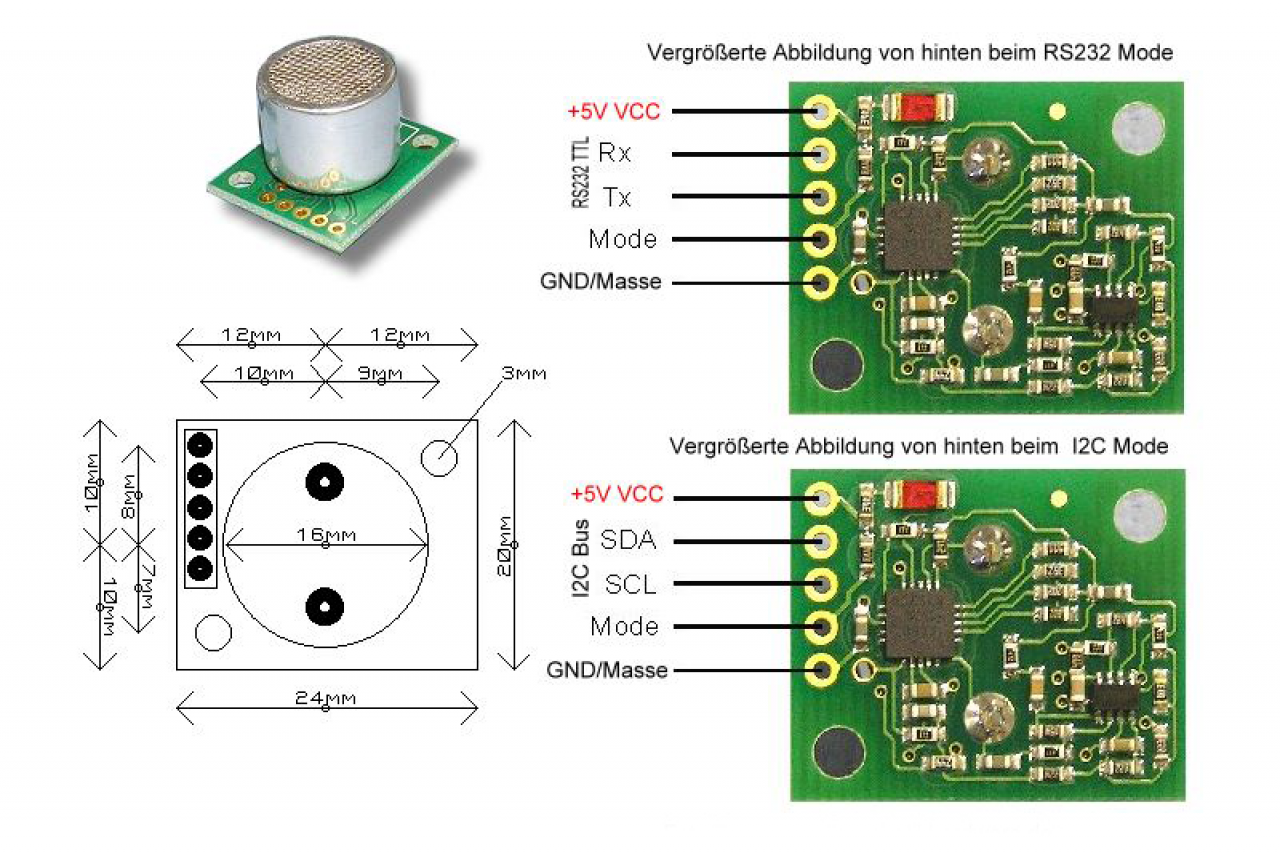
\includegraphics[width=0.5\textwidth, keepaspectratio]{images/wohlrab_srf02.png}
    \caption{Pinbelegung des Ultraschallsensors \cite{bild_ultraschall}}
    \label{fig:ultraschall_pinbelegung}
\end{figure}
Um die Funktionalität der Schaltung zu überprüfen und um eventuelle Anpassungen unkompliziert vornehmen zu können, wurde die Verbindung der Sensorpins mit den entsprechenden GPIO-Pins des Raspberry Pi zunächst mithilfe eines Breadboards realisiert.
In der finalen Ausführung wurden die Verbindungen durch individuelle Dupont-Crimp-Kabel ersetzt, um eine stabile und dauerhafte Verbindung sicherzustellen.

\subsection{Auslesen der Messwerte (Wohlrab)}

Der verwendete Ultraschallsensor verfügt über integrierte Funktionen, die direkt auf dem Sensorchip implementiert sind. 
Dadurch entfällt die Notwendigkeit, bestimmte grundlegende Mess- und Auswertungsroutinen softwareseitig umzusetzen, was den Entwicklungsaufwand erheblich reduziert.
Zur Initiierung einer Messung ist es ausreichend, eine definierte Startsequenz – zum Beispiel „0x51” für den Start einer Messung in Zentimetern – in das Befehlsregister zu schreiben. 
Dies löst automatisch den Messvorgang aus, der vollständig intern vom Sensor durchgeführt wird. Die Messdauer beträgt maximal 65 Mikrosekunden. 
Erst nach Ablauf dieser Zeitspanne kann das Messergebnis aus den zugehörigen Datenregistern ausgelesen werden.
Eine Besonderheit des Sensors ist die integrierte Kalibrierung sowie die automatische Umrechnung der Rohdaten in metrische Einheiten. 
Das Messergebnis wird direkt in Zentimetern bereitgestellt, sodass keine zusätzliche Nachbearbeitung durch die Software erforderlich ist.

\subsection{Verarbeiten der Messwerte (Wohlrab)}

Die Implementierung eines kontinuierlichen Datenstroms zur Ausgabe der Messwerte des Ultraschallsensors war technisch unkompliziert. 
Bereits nach der grundlegenden Anbindung des Sensors über die I²C-Schnittstelle konnten die gemessenen Distanzen problemlos in Echtzeit ausgelesen und weiterverarbeitet werden.
Bei der Analyse der ausgegebenen Werte zeigten sich jedoch charakteristische Abweichungen außerhalb des spezifizierten Messbereichs: 
Innerhalb eines bestimmten Entfernungsbereichs lieferte der Sensor präzise und nachvollziehbare Distanzangaben in Zentimetern. 
Wurde der Sensor jedoch in einem sehr kurzen Abstand angesteuert, traten fehlerhafte Werte auf – so stieg der ausgegebene Abstand trotz tatsächlicher Annäherung wieder an.
Ein vergleichbares Verhalten wurde bei Distanzen oberhalb von etwa vier Metern beobachtet. 
In diesem Fall lieferte der Sensor konstant den maximal darstellbaren Wert und reagierte nicht mehr auf Veränderungen der Umgebung. 
Der Sensor verblieb durchgehend in diesem Zustand, sodass keine neuen Messwerte generiert wurden.
Um diese Fehlfunktionen zu vermeiden, wurde eine softwareseitige Validierung implementiert, welche die Sensorwerte nur dann zur Weiterverarbeitung freigibt, wenn sie innerhalb des im Datenblatt spezifizierten Messbereichs liegen. 
Durch diese Einschränkung konnten die genannten Probleme vollständig behoben werden, sodass eine zuverlässige und konsistente Auswertung der Distanzmesswerte gewährleistet ist.
